% \documentclass[11pt,psfig]{article}
% \usepackage[T1]{fontenc}
% \usepackage{lmodern}
% \usepackage{amsmath,amssymb}
% \usepackage{bm}
% \usepackage{graphicx}
% \usepackage{xcolor}
% \usepackage{enumitem}
% \usepackage{array}
% \usepackage{booktabs}
% \usepackage[hidelinks]{hyperref}

% \oddsidemargin -0.04cm
% \evensidemargin -0.04cm
% \textwidth 16.59cm
% \textheight 21.94cm
% \topmargin -0.25cm
% \renewcommand{\baselinestretch}{1.35}

% \newcommand{\paperTitle}{MAML-Select: An Online Adaptive Client Selection Method for Federated Learning via Meta-Learning}
% \long\def\ReviewerHeading#1{%
%     \vspace{2em}
%     \begin{center}
%     {\bfseries\Large Response to Comments of #1}
%     \end{center}
%     \vspace{0.5em}
% }
% \long\def\ReviewerComment#1#2{%
%     \par\noindent\hspace{-0.65cm}{\bfseries #1:} {\itshape #2}\par\vspace{0.55em}
% }
% \long\def\ReviewerReply#1#2{%
%     \par\noindent\hspace{-0.65cm}{\bfseries #1:} {\normalfont #2}\par\vspace{1.0em}
% }

% \begin{document}

% \title{\small Response to Reviewers' Comments and Changes Incorporated in the Revised Manuscript\\[1.5em]
% {\Large \bfseries \paperTitle}\\[0.75em]
% (\textbf{Original Manuscript ID: TAI-2026-Mar-L-00619 })}
% \date{}
% \maketitle
% \vspace{-1.5em}

% We sincerely thank the Editor, the Associate Editor, and the anonymous Reviewers for their time and expert evaluation of our manuscript. Their detailed and constructive comments have been invaluable in significantly improving the overall quality of this paper. Based on this feedback, we have thoroughly revised the manuscript to enhance its clarity, technical completeness, evidentiary support, and presentation.

% Below, we provide a point-by-point response to each comment. For clarity, the Reviewers' original comments are formatted in \textit{italics}, followed immediately by our responses and the corresponding manuscript changes in normal text. Alongside this response letter, we have submitted both a clean version of the revised manuscript and a marked version with all modifications highlighted in blue.

% \ReviewerHeading{the Associate Editor}

% \ReviewerComment{Comment}{A strong revision stage is needed for this paper.}
% \ReviewerReply{Reply}{We are grateful to the Associate Editor for this guidance, and we have taken it to heart. We approached this round as a thorough, major revision rather than a light edit. We worked carefully through every concern the Reviewers raised, including the novelty, the theory, the breadth of the evaluation, the fairness analysis, the reproducibility, and the writing.

% The technical content is now considerably stronger. We sharpened how MAML-Select differs from reinforcement learning, contextual bandits, and meta-learning personalization, and we summarised this in a new comparison table (Table~I). To support the dynamic selection policy, we added theory where the original draft had none. We now prove a per-step descent property for both the inner and the outer adaptation steps (Statements~1 and~2 in Section~IV), together with a convergence rate (Corollary). We also broadened the experiments to three datasets of increasing difficulty, adding the harder CIFAR-100 task. The benchmark now covers eight methods across three seeds, and we report mean\,$\pm$\,standard deviation with paired-test significance. Beyond this, we added a complexity result (Eq.~(8)) and an $N$-scaling study up to $1000$ clients. We further added a two-dataset $\lambda$ sweep, inner-step, selector-width, and six-feature state ablations, fairness and coverage metrics with tier-level selection rates, and modelled energy and carbon under clearly stated device-tier assumptions.

% Alongside these additions, we gave the writing a careful pass. We shortened the longer sentences and regenerated every figure with larger, bolder fonts and clearer axes. We also specified the method and all hyper-parameters, so the results can be reproduced directly from the paper.

% The complete set of changes is listed in the Summary of Major Revisions below, and each point is then addressed in detail in the per-Reviewer responses that follow. We hope the revised manuscript now meets the strong-revision standard you asked for, and we sincerely appreciate the opportunity to improve it.}

% \vspace{1.5em}
% \begin{center}
% {\bfseries\Large Summary of Major Revisions}
% \end{center}

% \begin{itemize}[leftmargin=*,itemsep=0.35em]
%     \item \textbf{Sharpened novelty.} MAML-Select meta-learns the client-selection policy on the server. It re-adapts this policy every round. This is different from model personalization, reinforcement learning, and bandit selectors. We add a comparison table (Table~I).
%     \item \textbf{Local theory for a dynamic policy.} The selector is adapted online from changing feedback. So we add per-step descent statements and proofs for both the inner and the outer adaptation steps (Statements~1 and~2, Section~IV), together with a convergence rate (Corollary).
%     \item \textbf{Broader, harder evaluation.} We evaluate on Fashion-MNIST, CIFAR-10, and CIFAR-100. The setting is non-IID Dirichlet $\alpha=0.5$, $N=100$, $K=10$, and $E=5$. We use seeds $42$, $123$, and $2026$. We add FedGCS and CriticalFL, giving eight methods. We report mean\,$\pm$\,std with paired-test significance.
%     \item \textbf{Mechanism analysis.} We add a complexity result and an $N$-scaling study. We add a two-dataset $\lambda$ study, inner-step and selector-width ablations, and a six-feature state ablation. We add fairness and coverage metrics. We add modelled energy and carbon with stated device-tier values.
%     \item \textbf{Reproducibility.} We list all hyper-parameters. We give a full step-by-step pseudocode as Algorithm~S1 in Section~S5 of the Supplementary Material.
%     \item \textbf{Presentation.} We regenerated all figures with larger, bolder fonts and clearer axes. We shortened the Conclusion. We shortened the prose throughout.
% \end{itemize}

% \ReviewerHeading{Reviewer 1}

% \ReviewerComment{Comment 1}{Simplify long and complex sentences, especially in the Introduction and Related Work.}
% \ReviewerReply{Reply 1}{Agreeing with the Reviewer, we have now rewritten the manuscript with shorter sentences and a clearer flow. We made a full editing pass. It covers the Abstract, Impact Statement, Introduction, Related Work, System Model, Methodology, Evaluation, and Conclusion. We split long sentences into single-idea sentences. We also state the main motivation directly in the first paragraphs of the Introduction. Client utility changes during training. So a fixed selection rule becomes stale. A policy that re-adapts each round is therefore needed. We are grateful for this advice. It improved the readability of the whole paper, not only the two named sections.}

% \ReviewerComment{Comment 2}{Provide more implementation details, including optimizer type, learning rates, schedules, exact meta-policy architecture, initialization, random seeds, and code or detailed pseudocode.}
% \ReviewerReply{Reply 2}{We thank the Reviewer. Reproducibility is essential, and the method can now be reproduced from the paper. The meta-policy is a $6$-$64$-$64$-$1$ MLP with ReLU activations. It has $4{,}673$ trainable parameters. Local models use PyTorch default initialization. They use SGD with learning rate $0.01$, momentum $0.9$, weight decay $10^{-4}$, a constant schedule, batch size $32$, and $E=5$ local epochs. The MAML policy uses one inner step with $\beta=0.01$. The outer update uses Adam with $\eta=0.001$. The selector seed is fixed to $2026$. The data and training seeds are $42$, $123$, and $2026$. We also added a full step-by-step pseudocode. It is Algorithm~S1 (``MAML-Select (extended)'') in Section~S5 of the Supplementary Material. It expands Algorithm~1 of the main paper. It adds the state-feature construction, the cold-start rule, the exploration step, and the first-order inner and outer updates. It is the exact procedure used for every reported result. We also checked the two most specific design choices. A selector-width ablation varies the hidden width $h$ over $\{16,32,64,128\}$. This is $401$ to $17{,}537$ parameters. Final accuracy moves by less than about $0.6$ points. An inner-step ablation shows that one inner step is both the most accurate and the cheapest setting. Both results are in Section~V (Table~III), with a figure in Section~S3.}

% \ReviewerComment{Comment 3}{The accuracy gains are modest. Please justify why they are meaningful and identify scenarios where efficiency is prioritized.}
% \ReviewerReply{Reply 3}{We are grateful for this question. It goes to the heart of what the paper claims. We want to make the argument in plain terms, not only with numbers.

% In cross-device federated learning, the main limit at deployment is usually not the last fraction of a percent of accuracy. The main limit is compute, energy, battery, bandwidth, and the per-round deadline. A varied fleet of devices must meet these limits. Two points follow.

% First, an accuracy difference matters only when we compare it to its cost. We can trade a small, measured accuracy change for a large drop in compute and energy. That is a good trade whenever energy, carbon, or battery is the limiting budget.

% Second, where accuracy is not the bottleneck, MAML-Select matches the strongest baselines. So the efficiency gain comes almost for free. Our paired tests support this. Against FedGCS, the accuracy difference is not significant on CIFAR-10 ($p=0.10$) or CIFAR-100 ($p=0.49$). Against FedAvg, it is not significant on Fashion-MNIST ($p=0.84$).

% The efficiency benefit is consistent and significant. In federated learning, it is not only an environmental gain. A device that uses less energy per round can run more rounds before its battery or heat budget forces it to drop out. This raises its real availability. Over a full run, it also raises participation coverage. A synchronous round waits for the slowest selected client. So choosing feasible, low-cost clients also shortens each round. It reduces straggler delay. A selector that keeps accuracy within a small margin, while lowering compute, energy, and latency, improves the very limit that decides whether federated learning can run on a given fleet.

% The settings where this trade-off is the right one are concrete. They include battery and solar IoT and wearable sensors. They include mobile clients on metered, busy, or intermittent links. They include industrial IoT nodes with heat and power caps. They include carbon-aware (``Green-AI'') deployments. They include deadline-driven synchronous federated learning, where stragglers must be avoided. In all of these, a small, bounded accuracy cost for a large efficiency gain is the desired operating point.

% We are also careful not to over-claim. We present CIFAR-10 as the trade-off case. Its larger accuracy gap reflects the harder ResNet-18 task. There, one low-cost cohort per round can miss useful class variation. We describe MAML-Select as a resource-efficient selector with competitive accuracy, not dominant accuracy. This framing now appears in the Abstract, the Introduction, the Evaluation (the trade-off discussion and Fig.~3), and the Conclusion. The CIFAR-10 trade-off is stated openly.}

% \ReviewerHeading{Reviewer 2}

% \ReviewerComment{Comment 1}{Clarify the exact novelty compared with RL-based approaches, contextual bandits, and meta-learning-based personalization frameworks. Add a dedicated comparison table.}
% \ReviewerReply{Reply 1}{We thank the Reviewer. A clean separation from these three families is important. We now give it in both text and a table. The key difference is what is learned and when it is adapted.

% \noindent$\bullet$~\textbf{Reinforcement-learning selectors}, such as FAVOR with deep $Q$-learning, learn a long-horizon policy. They maximize a reward over many episodes. They need a lot of exploration. They must also assign credit across time. The learned controller is not re-fitted to the current situation just before each decision.

% \noindent$\bullet$~\textbf{Contextual and combinatorial bandits}, such as neural contextual bandits, learn a reward model from client features. They balance exploration and exploitation. They update reward estimates step by step. They do not take a gradient step on the scoring network from a fresh support set right before the next selection.

% \noindent$\bullet$~\textbf{Meta-learning personalization}, such as Per-FedAvg and pFedMe, uses MAML to adapt the client model to each client's data. There, the meta-learned object is the model.

% MAML-Select is different from all three. It meta-learns the initialization of the server-side ranking policy $\phi$. It then takes a first-order MAML inner step on that policy. The support set is the previous round's selected-client feedback. It then scores the current candidate pool, which is the query set, with the adapted policy. So the adapted object is the selector, not the client model. The adaptation is done every round by a gradient step on recent feedback. It is not a long-horizon RL update. It is not a slow bandit estimate. To our knowledge, this is the first method to frame per-round client selection as a meta-learning task with a clear support and query split and fast adaptation. Table~I now compares MAML-Select against representative methods from each family: system-aware selection (FedCS, TiFL), utility- and correlation-based selection (Oort, FedCor), reinforcement learning (FAVOR), neural contextual bandits (NCCB), joint-compression and generative or combinatorial selection (FedCG, FedGCS), critical-period scaling (CriticalFL), robust and fair selection (Kazemi et al., Vox Populi), and meta-learning personalization (Per-FedAvg). It uses four columns: primary objective, adaptation mechanism, selection complexity or dominant operation, and optimization strategy. This directly contrasts the three families the Reviewer names: FAVOR for reinforcement learning, the neural contextual bandit for bandits, and Per-FedAvg for meta-learning personalization, the last of which adapts the client model rather than the selector. The ``Difference from prior work'' paragraph in Related Work and the Introduction also state this directly.}

% \ReviewerComment{Comment 2}{The manuscript has empirical evaluation only. There is no convergence proof or theoretical justification for non-stationary adaptation.}
% \ReviewerReply{Reply 2}{We thank the Reviewer for pressing on the theory. This is a fair and important point, and we have strengthened the analysis well beyond a disclaimer. The selection policy in MAML-Select is dynamic. It is re-adapted every round from fresh, changing feedback. So the right object to analyze is the per-round adaptation. We now prove a descent property for \emph{both} of its steps, add a convergence rate, and verify both empirically.

% \emph{Inner step (Statement~1).} Let $g_t(\phi)=\mathcal{L}_{sup}(h_\phi;\mathcal{D}_{sup}(t))$. If $g_t$ is $L$-smooth and $0<\beta<2/L$, the inner update satisfies $g_t(\phi'_t)\le g_t(\phi_t)-\beta(1-\tfrac{L\beta}{2})\lVert\nabla g_t(\phi_t)\rVert_2^2$. So one support step does not increase, and generically decreases, the round's selector loss before ranking.

% \emph{Outer step (Statement~2).} This is the part the Reviewer notes was missing, and we now prove it. Let $q_t(\phi)=\mathcal{L}_{query}(h_\phi)$ be $L_q$-smooth and $0<\eta\le 1/L_q$. The first-order meta-update obeys $q_t(\phi_{t+1})\le q_t(\phi_t)-\tfrac{\eta}{2}\lVert\nabla q_t(\phi_t)\rVert_2^2+\tfrac{\eta}{2}\delta_t^2$, where $\delta_t\le L_q\beta\lVert\nabla g_t(\phi_t)\rVert_2$ is the first-order approximation error. So the meta-update decreases the query objective, up to a correction of order $\beta^2$. With $\beta=0.01$ this correction is negligible. This gives the outer loop a per-step descent guarantee and makes the first-order approximation rigorous.

% \emph{Rate (Corollary).} Summing Statement~2 over rounds gives $\min_{t\le T}\lVert\nabla q(\phi_t)\rVert_2^2\le \tfrac{2(q(\phi_1)-q^\star)}{\eta T}+\tfrac1T\sum_t\delta_t^2$. So the meta-policy reaches an $\mathcal{O}(\beta^2)$-approximate stationary point at rate $\mathcal{O}(1/(\eta T))$.

% \emph{Empirical check.} Because the query target drifts slowly, we also verify both properties empirically. The Supplementary Material (Section~S6) plots, over a full run on each dataset, the inner-step descent (at or below zero in $100\%$ of rounds on all three datasets), the query objective (decreasing then stabilizing), and the meta-update magnitude (shrinking and settling). The global model also converges, as the accuracy and loss curves in the main paper show.

% Statements~1 and~2 appear in Section~IV, after the inner-loop equation~(5) and the outer-loop equation~(7). On the convergence theory, one problem remains open: a closed-form \emph{global} guarantee for the entire FL loop under adaptive partial participation, where the selection distribution, the global model, and the data partition all evolve together.}

% \ReviewerComment{Comment 3}{Explain the manually chosen trade-off parameter $\lambda$ and evaluate sensitivity.}
% \ReviewerReply{Reply 3}{We appreciate the request for both an explanation and evidence. We have strengthened both.

% \emph{What $\lambda$ is.} $\lambda$ is the price the selector puts on latency, compared to learning progress. It enters the per-client cost in Eq.~(4): $c_{i,t}=\lambda\,\max(0,T_{i,t}-T_{target})-\Delta_{i,t}$. Here $\Delta_{i,t}$ is the observed local loss reduction. At $\lambda=0$, the selector is purely utility-driven. It then ignores latency. As $\lambda$ grows, it prefers feasible, low-cost clients more and more. So $\lambda$ moves the operating point along the efficiency and accuracy frontier. It is not a tuned accuracy knob. It is a budget dial for the deployer. It is also defined in the System Model (Eq.~(3)).

% \emph{Evidence.} The study now sweeps $\lambda$ over $\{0.1,0.5,1.0,5.0\}$. It does this on both Fashion-MNIST and CIFAR-10 (Fig.~5, two panels, plus a two-dataset table). Before, the sweep was on Fashion-MNIST alone. On Fashion-MNIST, accuracy is nearly flat. It changes by about one point across the range. So the cost term can be raised almost for free. On CIFAR-10, the trade-off is sharper. Accuracy falls from $64.9\%$ at $\lambda=0.1$ to $56.3\%$ at $\lambda=5$. At the same time, compute drops by about $26\%$ and modelled energy by about $30\%$. The reason is that ResNet-18 training is costly. Strong cost-minimization can drop class-diverse but costly clients. Fairness also drops at large $\lambda$.

% \emph{Why $\lambda=0.5$.} It sits at the knee of this frontier. It keeps accuracy close to the best setting. It still gives a clear compute and energy reduction. It also avoids the sharp fairness drop seen at $\lambda\ge1$. We use $0.5$ as a balanced default. We report the full sweep so a reader can pick another point for a different budget.}

% \ReviewerComment{Comment 4}{The experimental validation is limited to small-scale datasets. Add larger or more realistic FL benchmarks.}
% \ReviewerReply{Reply 4}{We understand the concern. We address it in two ways. We add a harder benchmark, and we add a clear scalability argument. We are also honest about what we did and did not run.

% First, we added CIFAR-100 with ResNet-18. It is a $100$-class non-IID task. It is much harder than Fashion-MNIST and CIFAR-10. It stresses the selector under fine-grained class heterogeneity. MAML-Select stays competitive with the strongest baselines there. It also keeps its efficiency advantage.

% Second, the concern is really about scale. So we added a selector-overhead scaling study (Fig.~4). It uses $N$ over $\{20,40,80,100,200,500,1000\}$ with $K/N=0.1$. We also added a complexity result (Eq.~(8)). The per-round server cost is $\mathcal{O}(NP+N\log K+2KP)$. This is linear in the client-pool size $N$ for a fixed policy size $P$ and cohort $K$. The measured overhead stays nearly flat, at about $20$ to $26$~ms per round, even as $N$ grows fifty-fold to $1000$. So the selector is cheap to run at large pools, and the trend is now measured rather than extrapolated. So the method is ready, in compute terms, for much larger pools.

% We agree that very large, naturally-federated datasets are valuable. Examples are LEAF-style FEMNIST or Shakespeare, or pools with thousands of clients. We mark them as future work in the Conclusion. Our contribution is the selection mechanism and its resource behaviour. We validate it across three datasets of growing difficulty and an explicit $N$-scaling study. We chose to report only experiments run at the full protocol with repeated seeds. We did not want to add a benchmark we could not validate to the same standard. The Evaluation now covers Fashion-MNIST, CIFAR-10, and CIFAR-100. The scaling study and complexity result are in Section~V.}

% \ReviewerComment{Comment 5}{Include standard deviation across multiple runs and statistical significance analysis.}
% \ReviewerReply{Reply 5}{Reporting variability and significance is essential for a fair comparison. The revised paper now does both. Every entry in the main benchmark table (Table~II) is a mean\,$\pm$\,standard deviation. It is over the three seeds $42$, $123$, and $2026$. The selector seed is held fixed. So the reported variance reflects model-training and data-partition randomness. It does not reflect selector re-initialization.

% For significance, we use paired $t$-tests over shared seeds. Each method is evaluated on the same seed. So the test controls for partition and initialization effects. The resource reductions versus FedAvg are significant on all three datasets. The TFLOP $p$-values are $0.009$, $0.002$, and $0.012$. The energy and carbon $p$-values are $0.007$, $0.001$, and $0.003$. These are for Fashion-MNIST, CIFAR-10, and CIFAR-100.

% For accuracy, we report the paired comparison honestly, not selectively. Against FedGCS, the difference is not significant on CIFAR-10 ($p=0.10$) or CIFAR-100 ($p=0.49$). Against FedAvg, it is not significant on Fashion-MNIST ($p=0.84$). This is exactly why we frame the result as an efficiency gain at competitive accuracy. The full paired tests and standardized effect sizes are also in Section~S2 of the Supplementary Material.}

% \ReviewerComment{Comment 6}{Evaluate fairness across heterogeneous clients using participation fairness, client coverage, or tier-level selection rates.}
% \ReviewerReply{Reply 6}{We have made the fairness analysis more complete and, we hope, clearer. We report two quantities. They measure different things.

% Coverage is the breadth of participation. It is the percentage of clients selected at least once during a run: $\mathrm{Cov}=\tfrac{100}{N}\,|\{i:\sum_t a_{i,t}\ge1\}|$. It answers one question. Is any client left out forever?

% Jain's index measures how evenly participation is spread. It is $J=(\sum_i p_i)^2/(N\sum_i p_i^2)$, over the per-client selection counts $p_i$. A value of $J=1$ means perfectly even participation.

% MAML-Select reaches $100\%$ coverage on all three datasets. So no client is ever starved. Its Jain index is $0.61$ to $0.78$. This is more concentrated than random selection. This is the expected and intended result of utility-aware selection. The policy prefers high-utility, low-cost clients. So the counts are less even. But the staleness and frequency features keep the concentration bounded. They prevent permanent exclusion. The contrast with the system-aware baselines is the key point. FedCS, Oort, and TiFL reach only $10$ to $12\%$ coverage. Their Jain index is about $0.10$. They keep selecting a small fast subset and never include slow clients. So MAML-Select is far more inclusive than those selectors. It is also more efficient. We do not claim it is the fairest selector overall. FedAvg and FedGCS have a higher Jain index. So our claim is precise. MAML-Select gives full coverage with a much better compute and energy profile. Table~II reports Jain and coverage for every method. The Evaluation discusses the coverage versus evenness point directly. We also report the tier-level selection rates the Reviewer asks for (Supplementary Material, Section~S2). The device pool is $20\%$ slow (Tier~1), $50\%$ medium (Tier~2), and $30\%$ fast (Tier~3), so a proportional selector reads $0.20/0.50/0.30$. The tier pattern matches the coverage result. FedCS selects no slow-tier client at all ($0.00$) and sends $80$ to $83\%$ of its picks to the fast tier. MAML-Select shifts toward faster tiers to save latency and energy (fast-tier rate $0.44$ to $0.49$), but it still selects the slow tier ($0.09$) and keeps $100\%$ coverage. So MAML-Select is cost-aware at the tier level without abandoning any tier.}

% \ReviewerComment{Comment 7}{The claims regarding energy efficiency and Green AI are indirect. Moderate the wording or provide stronger evidence.}
% \ReviewerReply{Reply 7}{We agree that the basis of the energy claims must be clear. We made the measurement model explicit. We also kept the efficiency evidence. The revised paper reports TFLOPs. It also reports model-based energy and carbon estimates. These come from stated client-tier values. Tier~1 uses $4$~W power and an $18$~Wh battery. Tier~2 uses $7$~W and $30$~Wh. Tier~3 uses $12$~W and $48$~Wh. Carbon uses $475$~gCO$_2$e/kWh. Energy and carbon are defined by explicit equations in Section~V. The same accounting model is applied to every method. So the comparison isolates the effect of client selection, not of an outside estimator. We also call these values ``modelled'' estimates throughout. We cite CodeCarbon~v2.4.1 for the carbon metadata and units. We believe this gives a stronger and reproducible basis than an unqualified Green-AI claim.}

% \ReviewerComment{Comment 8}{Justify the six state features and provide an ablation study.}
% \ReviewerReply{Reply 8}{We expanded both the justification and the ablation. The state vector $\bm{s}_{i,t}$ has six entries. We group them by the signal each one carries.

% \emph{Statistical utility.} The local training loss $\hat{L}_{i,t}$ tells us if the client still has useful gradients. The gradient norm $\lVert\nabla F_i\rVert_2$ tells us the size and value of the update.

% \emph{System feasibility.} The estimated latency $\hat{T}_{i,t}$ tells us the straggler and round-time risk. The battery level $b_{i,t}$ tells us the energy feasibility and the drop-out risk.

% \emph{Participation balance.} The selection frequency $q_{i,t}$ helps avoid over-using a few clients. The staleness $\tau_{i,t}$, the rounds since last selected, helps avoid starving clients.

% Together, these six cover the statistical, system, and fairness signals a selector must weigh. They also stay compact and privacy-preserving. No raw client data leaves the device. Only the six scalars and a scalar cost are shared.

% The leave-one-feature-out ablation is in Table~IV (Fashion-MNIST). Final accuracy moves by less than about $0.35$ percentage points under any single removal. So the policy is not sensitive to one missing input. The largest accuracy drop comes from removing the battery feature, and removing latency or loss also lowers accuracy. This confirms that both system status and learning feedback are truly used. Removing the frequency feature instead raises accuracy slightly, but it lowers the Jain index the most, from $0.78$ to $0.65$. So the participation features mainly protect fairness, not accuracy. We keep all six on purpose, rather than chase a small accuracy gain. The per-feature reasons are in the State-Space paragraph (Section~IV). The ablation is in Section~V (Table~IV). A companion figure is in Section~S3.}

% \ReviewerComment{Comment 9}{Fig. 2 has small font sizes and unclear axis scaling.}
% \ReviewerReply{Reply 9}{Thank you for catching this. Legibility matters, and we rebuilt the figures. All figures were regenerated with much larger, bold fonts, boxed axes, clearer legends, and consistent placement. The convergence figure (Fig.~2) is now at full column width. It reports CIFAR-100 test accuracy, weighted precision, cumulative modelled carbon, and test loss over rounds. So the comparison is no longer a single efficiency curve. It is now a multi-metric, round-wise view across all eight methods. We also enlarged the axis ranges and tick labels. So the curves and scales read clearly in print.}

% \ReviewerComment{Comment 10}{The definition of ``Time (Units)'' is unclear.}
% \ReviewerReply{Reply 10}{We agree the abstract time unit was unclear. We removed it. The main results table (Table~II) now reports only well-defined quantities. These are accuracy, weighted precision, recall, F1, TFLOPs, modelled energy (Wh), modelled carbon (gCO$_2$e), Jain fairness, and coverage. Each one is defined in the Evaluation. Where round latency matters, we describe it through the straggler-bound round time in the System Model, not an unlabeled time unit.}

% \ReviewerComment{Comment 11}{Include recent baselines such as CriticalFL and FedGCS.}
% \ReviewerReply{Reply 11}{We added both methods. FedGCS uses generative client-combination search. CriticalFL uses critical-period cohort scaling. Both are now in the benchmark table, the related-work discussion, and the main evidence figures. The comparison now has eight methods in total. These are FedAvg, FedCS, Oort, TiFL, FedCor, FedGCS, CriticalFL, and the proposed MAML-Select. They span random, system-aware, utility-aware, correlation-based, generative, and critical-period selection. So the evaluation now places MAML-Select against current state-of-the-art selectors.}

% \ReviewerComment{Comment 12}{Proofread the manuscript for grammar, punctuation, and sentence structure.}
% \ReviewerReply{Reply 12}{We completed a full proofreading and prose pass over the whole manuscript. We shortened sentences. We fixed grammar and punctuation. We removed vague or unsupported claims. The Abstract, Impact Statement, Introduction, Related Work, Methodology, Evaluation, and Conclusion were all edited for clarity and consistent terms.}

% \ReviewerHeading{Reviewer 3}

% \ReviewerComment{Comment 1}{The motivation is not clear.}
% \ReviewerReply{Reply 1}{We thank the Reviewer and have sharpened the motivation. The central issue is that client utility in federated learning is non-stationary. A client that is useful in one round may be less useful later. The reason is that many things change during training. The global model changes. The local loss changes. The device latency and battery state change. The participation history also changes. A fixed scoring rule cannot track this drift. Re-training a heavy controller from scratch each round is also impractical at the edge. MAML-Select solves this by meta-learning a ranking policy. Its initialization can be adapted with a single gradient step. This step uses the most recent round's feedback, just before the next decision. So it is fast enough to run every round. It is also responsive to the changing utility. This motivation now opens the Abstract and the Introduction. It frames the contributions.}

% \ReviewerComment{Comment 2}{Highlight the novelty and main contribution.}
% \ReviewerReply{Reply 2}{We have stated the contribution more precisely. We also gave it a clear three-part structure. The novelty is methodological. To our knowledge, this is the first method to treat per-round federated client selection as a meta-learning task, and to solve it with first-order MAML. Three elements are new together. First, the meta-learned object is the server-side ranking policy, not the client model. So this is not personalization. Second, each round is treated as a task. It has an explicit support set, which is the previous round's selected-client feedback. It also has a query set, which is the current candidate pool. So the policy is re-fitted by a gradient step right before every selection. It is not learned once, as in RL. It is not updated only as reward estimates, as in bandits. Third, the cost that supervises the policy joins learning progress and system latency. It does so through one clear parameter, $\lambda$. This gives a tunable efficiency and accuracy operating point. The Introduction, the ``Difference from prior work'' paragraph in Related Work, and Table~I now make this three-part contribution explicit. It is the same distinction summarized in our reply to Reviewer~2, Comment~1.}

% \ReviewerComment{Comment 3}{Add appropriate constraints to the problem formulation.}
% \ReviewerReply{Reply 3}{We added the missing constraints, so the selection problem is fully specified. The System Model now introduces the per-round available-client set $\mathcal{A}_t$. It adds binary decision variables $a_{i,t}\in\{0,1\}$. It adds the cohort-size constraint $\sum_i a_{i,t}=K$. It adds the availability constraint $a_{i,t}\le\mathbf{1}\{i\in\mathcal{A}_t\}$, with $\mathcal{S}_t=\{i:a_{i,t}=1\}$. These appear in the constrained problem of Eq.~(3). This makes clear that selection is a combinatorial choice. It is limited by availability and made over a small feasible cohort.}

% \ReviewerComment{Comment 4}{Why is only one method considered as a baseline? Consider at least two more baselines.}
% \ReviewerReply{Reply 4}{The revised evaluation compares MAML-Select against seven baselines. They span the major design philosophies. FedAvg is random. FedCS is system-aware and deadline-constrained. Oort uses utility-based importance sampling. TiFL is tier-based. FedCor is correlation-based, using Gaussian Processes. FedGCS is generative. CriticalFL uses critical-period cohort scaling. All appear in Table~II, the related-work comparison (Table~I), and the main evidence figures. So the comparison is now broad, not single-baseline.}

% \ReviewerComment{Comment 5}{Provide more simulation results to ensure effectiveness.}
% \ReviewerReply{Reply 5}{We expanded the empirical evidence a great deal. The revised paper covers three datasets. Fashion-MNIST and CIFAR-10 run for $200$ rounds. CIFAR-100 runs for $150$ rounds. It covers eight methods and three seeds, with mean\,$\pm$\,std and paired-test significance. It adds fairness and coverage metrics. It adds a two-dataset $\lambda$ sweep. It adds inner-step and selector-width ablations. It adds a six-feature state ablation. It adds modelled energy and carbon. It adds a selector-overhead scaling study with a supporting complexity result. The reported metrics include accuracy, precision, recall, F1, compute, energy, fairness, coverage, sensitivity, ablation, and server-side overhead. More tables and figures are in the Supplementary Material (Sections~S2 to~S5).}

% \ReviewerComment{Comment 6}{Remove references from the conclusion and write the conclusion as a concise single paragraph.}
% \ReviewerReply{Reply 6}{We followed this suggestion. The Conclusion is now a single concise paragraph with no citations. It summarizes the method and findings. It ends with a short statement of future directions. These are a broader evaluation across heterogeneity levels, client-pool sizes, and naturally federated benchmarks, an asynchronous extension, and a differentially private treatment of the client-state vector.}

% \ReviewerHeading{Reviewer 4}

% \ReviewerComment{Comment 1}{Correct the Impact Statement wording for heterogeneous environments and industrial Internet of Things.}
% \ReviewerReply{Reply 1}{We adopted the suggested terms and moderated the impact claims. The Impact Statement now uses ``heterogeneous environments'' and the ``industrial Internet of Things.'' It also states clearly that the reported energy and carbon figures are modelled estimates. They follow the stated device-tier and grid-intensity assumptions. So the impact is framed transparently, not as a fixed energy guarantee.}

% \ReviewerComment{Comment 2}{Improve long sentences, grammar, and proofreading throughout the manuscript.}
% \ReviewerReply{Reply 2}{We revised the manuscript for shorter, clearer prose. We also corrected grammar and punctuation throughout. The Abstract, Impact Statement, Introduction, Related Work, Methodology, Evaluation, and Conclusion were all edited. This adds to the proofreading pass noted in our reply to Reviewer~1, Comment~1, and Reviewer~2, Comment~12.}

% \ReviewerComment{Comment 3}{Update the literature review with recent and related papers.}
% \ReviewerReply{Reply 3}{We updated the Related Work and focused the bibliography. The revised paper keeps the canonical algorithm references for every compared method. It also adds recent, relevant work. This covers robust selection, adaptive straggler handling, inclusive participation, asynchronous heterogeneity, and non-IID federated learning. So the discussion reflects the current state of the field. It also stays focused on client selection.}

% \ReviewerComment{Comment 4}{Include a comparison table with previous state-of-the-art works.}
% \ReviewerReply{Reply 4}{We added the requested table. Table~I compares representative client-selection and meta-learning approaches against MAML-Select. It uses four columns: primary objective, adaptation mechanism, selection complexity or dominant server-side operation, and optimization strategy. This makes the method's position relative to prior work clear at a glance.}

% \ReviewerComment{Comment 5}{Make the Conclusion and Future Work section accurate and concise. Avoid too many citations.}
% \ReviewerReply{Reply 5}{We revised the Conclusion to a single concise paragraph without citations. It ends with a short, accurate statement of future directions. These are a broader evaluation across heterogeneity levels, client-pool sizes, and naturally federated benchmarks, an asynchronous extension, and a differentially-private treatment of the client-state vector.}

% \ReviewerComment{Comment 6}{Fig. 2 requires clarification, justification, and a clearer comparison with other schemes.}
% \ReviewerReply{Reply 6}{The original single-curve figure has been replaced by clearer, multi-metric evidence. The convergence figure (Fig.~2) now reports CIFAR-100 accuracy, precision, cumulative modelled carbon, and test loss over rounds, for all eight methods. The efficiency and accuracy trade-off figure (Fig.~3) places MAML-Select directly against every baseline. It uses final accuracy and training compute relative to FedAvg. Together with the $\lambda$-sensitivity, feature-ablation, and selector-scaling figures, the visual evidence now justifies the design choices. It also compares schemes clearly. The fonts are larger and bold, and the axes are labeled.}


% \end{document}
% Preview source code

%% LyX 2.5.1 created this file.  For more info, see https://www.lyx.org/.
%% Do not edit unless you really know what you are doing.
\documentclass[10pt]{article}
\usepackage{lmodern}
\usepackage{lmodern}
\usepackage[LGR,T1]{fontenc}
\usepackage[utf8]{inputenc}
\usepackage{microtype}
\usepackage{enumitem}
\usepackage{bm}
\usepackage{amsmath}
\usepackage{amssymb}
\usepackage[bookmarks=false,
 breaklinks=false,pdfborder={0 0 1},backref=false,colorlinks=false]
 {hyperref}

\makeatletter

%%%%%%%%%%%%%%%%%%%%%%%%%%%%%% LyX specific LaTeX commands.
\DeclareRobustCommand{\greektext}{%
  \fontencoding{LGR}\selectfont\def\encodingdefault{LGR}}
\DeclareRobustCommand{\textgreek}[1]{\leavevmode{\greektext #1}}


%%%%%%%%%%%%%%%%%%%%%%%%%%%%%% Textclass specific LaTeX commands.
\newlength{\lyxlabelwidth}      % auxiliary length 

\@ifundefined{date}{}{\date{}}
%%%%%%%%%%%%%%%%%%%%%%%%%%%%%% User specified LaTeX commands.


\usepackage{bm}
\usepackage{graphicx}
\usepackage{xcolor}
\usepackage{array}
\usepackage{booktabs}


\oddsidemargin -0.04cm
\evensidemargin -0.04cm
\textwidth 16.59cm
\textheight 21.94cm
\topmargin -0.25cm
\renewcommand{\baselinestretch}{1.35}
\setlength{\parindent}{0pt}
\setlength{\parskip}{0.55em plus 0.1em minus 0.1em}

\newcommand{\paperTitle}{MAML-Select: An Online Adaptive Client Selection Method for Federated Learning via Meta-Learning}
\long\def\ReviewerHeading#1{%
    \vspace{2em}
    \begin{center}
    {\bfseries\Large Response to Comments of #1}
    \end{center}
    \vspace{0.5em}
}
\long\def\ReviewerComment#1#2{%
    \par\noindent\hspace{-0.65cm}{\bfseries #1:} {\itshape #2}\par\vspace{0.55em}
}
\long\def\ReviewerReply#1#2{%
    \par\noindent\hspace{-0.65cm}{\bfseries #1:} {\normalfont #2}\par\vspace{1.0em}
}

\makeatother

\begin{document}
\title{
\small Response to Reviewers' Comments and Changes Incorporated in the Revised Manuscript \\
\vspace{1em}
{\Large \bf MAML-Select: An Online Adaptive Client Selection Method for Federated Learning via Meta-Learning} \\
(\textbf{Original Manuscript ID: TAI-2026-Mar-L-00619})
}
\date{}
\maketitle

\vspace{-3em}

We sincerely thank the Editor, Associate Editor, and all four anonymous Reviewers for their valuable time and effort in evaluating our manuscript. We are also thankful to all of you for the detailed and constructive feedback on our manuscript. The comments provided were extremely valuable and have helped us significantly improve the quality, clarity, and technical depth of our work. In the revised version, we have carefully
addressed all the raised concerns. {\color{blue}All changes made in response to the Reviewers’ comments have been clearly highlighted in blue, as per the journal's guidelines}. Below, we provide a detailed point-by-point response to each comment. Please note that the Reviewers' comments are \textit{italicized}, followed by our responses in normal font.  Along with this letter we submit (a) a clean version of the revised manuscript, (b) coloured marked version of the revised manuscript, in which changes are highlighted, and (c) a supplementary file supporting the justifications provided in the replies to Reviewers' comments.\\

\hspace{0.75cm}{\bf {\Large {~~~~~~~~~~~~Response to Comments of Associate Editor}}}

\noindent
\textbf{Comment:} \textit{{A strong revision stage is needed for this paper.}}\\
\noindent
\textbf{Reply:} {We thank the Associate Editor for providing us with an opportunity to revise and resubmit the manuscript. We have carefully revised the manuscript and all the necessary changes are incorporated in the revised manuscript. The changes made are highlighted in blue in the revised manuscript. The technical content has been strengthened on every axis raised by the Reviewers. We sharpen the novelty against reinforcement-learning, contextual-bandit, and meta-learning personalization methods, and add a dedicated comparison table (Table~I). We add a theoretical justification for the per-round adaptation, namely two descent lemmas and a convergence corollary (Section~IV). We broaden the evaluation to a harder benchmark (CIFAR-100) and to eight methods over three seeds, now reported as mean\,$\pm$\,standard deviation with paired-test significance. We have added a complexity result and an $N$-scaling study up to $1000$ clients, a two-dataset $\lambda$ sweep, inner-step, selector-width, and six-feature ablations, fairness and coverage metrics with tier-level rates, and modelled energy efficiency under stated device-tier assumptions. We also specify the full implementation for reproducibility and rewrite the manuscript for clarity. The detailed changes are described in the per-Reviewer responses below.}\\

\hspace{0.75cm}{\bf {\Large {~~~~~~~~~~~~Response to Comments of Reviewer 1}}}

\noindent
\textbf{Comment 1:} \textit{Simplify long and complex sentences, especially in the Introduction and Related Work.} \\
\textbf{Reply 1:} We are thankful to the Reviewer for his/her valuable suggestion to improve the readability of the revised manuscript. As per your suggestion, we have now
rewritten the manuscript with simplified sentences.
We made a full editing pass throughout the manuscript. In particular, please refer the Introduction and Related Work section of the revised manuscript.

%As a concrete example, the Related Work has been reorganized into three short, labelled subsections (system-aware, data/utility-based, and learning-based selection), each written as a few single-idea sentences in place of the earlier long compound sentences. In the Introduction, likewise, the points about client heterogeneity and the selection problem are now stated as separate short sentences rather than one long clause.}\\

\noindent
\textbf{Comment 2:} \textit{Provide more implementation details, including optimizer type, learning rates, schedules, exact meta-policy
architecture, initialization, random seeds, and code or detailed pseudocode.} \\
\noindent
\textbf{Reply 2:} {We thank the Reviewer for asking more details with respect to implementation of the proposed method. Towards reproducibility, more details are now added in the Sections IV and V of the revised
paper. In particular, the meta-policy is a $6$-$64$-$64$-$1$ MLP with ReLU activations. It has $4{,}673$ trainable parameters. Local models
use PyTorch default initialization, and SGD is used with learning
rate $0.01$. Please note that momentum is $0.9$, weight decay has a value of $10^{-4}$, while a constant schedule is used with a batch size $32$, and $E=5$ local epochs. The MAML policy
uses one inner step with $\beta=0.01$. The outer update uses Adam
with $\eta=0.001$. The selector seed is fixed to $2026$. The tests use seeds $42$, $123$, and $2026$. We also added a
full step-by-step pseudocode for your kind reference in Algorithm~S1 (``MAML-Select
(extended)'') in Section~S5 in the Supplementary Material.


}\\

\noindent
\textbf{Comment 3:} \textit{The accuracy gains are modest. Please
justify why they are meaningful and identify scenarios where efficiency is prioritized.} \\
\noindent
\textbf{Reply 3:} We thank the Reviewer for asking the justification. We would like to clarify that, in cross-device
federated learning, test accuracy (averaged across clients) is not
the only criteria, which define the superiority of the federated learning
algorithm. Other factors include computational cost, energy efficiency,
bandwidth, timely completion of updates via per-round deadline. In
the revised manuscript, we have now investigated not only from the
accuracy point of view, but also from other important factors defining
the learning algorithm. Though it is evident that the testing accuracy
contributes significantly to the cost, however, a small change in
accuracy can contribute to a large cost, especially in terms of energy, time, and bandwidth.
In the revised work, MAML-select matches with the strongest baselines. That is, with the proposed client selection policy, there is a significant advantage in terms of communication-costs and computational-overhead cost, when compared with the baselines without client selection or a stationary client selection policy. Therefore, even if there is
a modest advantage in terms of accuracy, we are gaining in terms of communication-cost and computational-costs. In the revised manuscript, these costs have been analyzed, and their improvement over baselines have been presented. 

Moreover, a synchronous round waits for the slowest selected client
to participate. However, with a client selection approach, low-cost
clients can shorten the update time of rounds, and lead to faster
learning, that is, straggler can be omitted. Therefore, one can describe
MAML-Select as a resource-efficient selector with competitive accuracy,
not dominant accuracy. 

To make the cost advantage concrete, Fig.~3(a) of the revised manuscript reports the accuracy--compute trade-off, plotting final accuracy against cumulative training compute (in TFLOPs) relative to FedAvg for every method, while the corresponding per-round latency and modelled-energy values are listed in Table~II of the revised manuscript. Please refer Fig 3(a) and Table II of the revised manuscript.\\


\hspace{0.75cm}{\bf {\Large {~~~~~~~~~~~~Response to Comments of Reviewer 2}}}

\noindent

\textbf{Comment 1:} \textit{Clarify the exact novelty compared
with RL-based approaches, contextual bandits, and meta-learning-based
personalization frameworks. Add a dedicated comparison table.} \\
\noindent
\textbf{Reply 1:} {We thank the Reviewer for recommending additional comparison frameworks. In response, we have included and discussed the following representative client-selection frameworks in the revised manuscript: 
\begin{itemize}
\item \textbf{Reinforcement-learning selectors}, such as FAVOR [14]
with deep $Q$-learning, learn a long-horizon policy. They maximize
a reward over many episodes. They need a lot of exploration. They
must also assign credit across time. The learned controller is not
re-fitted to the current situation just before each decision. Even
if we compare, it can be clearly seen that the deep RL approach will
be needing much more number of rounds, computational, storage, and
communication cost, due to ``exploration''.
\item \textbf{Contextual and combinatorial bandits}, such as neural contextual
bandits (NCCB) [15], learn a reward model from client features. These class of
approaches are similar to RL approaches, and balance exploration and
exploitation. Reward estimates are updated step by step, over many
episodes. They do not take a gradient step on the scoring network
from a fresh support set right before the next selection. 
\item \textbf{Meta-learning personalization}, such as Per-FedAvg [18] and pFedMe,
uses MAML to adapt the client model to each client's data. There,
the meta-learned object is the model, not the client selection policy.
\end{itemize}
MAML-Select is different from all three. It meta-learns the initialization
of the server-side ranking policy $\phi$. It then takes a first-order
MAML inner step on that policy. The support set is the previous round's
selected-client feedback. It then scores the current candidate pool,
which is the query set, with the adapted policy. Thus, the adapted
object is the selector, not the client model. The adaptation is done
every round by a gradient step on recent feedback. In other words,
a long-horizon RL update or a exploration based bandit estimate are
much different from the proposed solution for the client selection.
Each client is either included or excluded in a given round. Thus,
in a given round, the client selection problem is np-hard combinatorial
problem, whose space increases exponentially with the increase in
the number of users. Therefore, the RL methods will become infeasible,
as the number of clients will increase. In other words, the suggested
methods are not scalable in this context. 

In the revised manuscript, the Table~I now compares MAML-Select against representative methods from each family: system-aware selection (FedCS [7], TiFL [8]), utility- and correlation-based
selection (Oort [9], FedCor [10]), reinforcement learning (FAVOR [14]), neural contextual bandits (NCCB [15]), joint-compression and generative or combinatorial selection (FedCG [11], FedGCS [13]), critical-period scaling (CriticalFL [12]), robust
and fair selection (Kazemi et al.\ [16], Vox Populi [20]), and meta-learning personalization (Per-FedAvg [18]).
The references used in the aforementioned discussion and their numbering is as per the revised manuscript.

% The table is organized around the dimension that separates these methods from ours, namely what each one adapts and how often it does so. It uses four columns: primary objective, adaptation mechanism,
% selection complexity or dominant operation, and optimization strategy.
% This directly contrasts the three families the Reviewer names: FAVOR
% for reinforcement learning, the neural contextual bandit for bandits,
% and Per-FedAvg for meta-learning personalization, the last of which
% adapts the client model rather than the selector. The ``Difference
% from prior work'' paragraph in Related Work and the Introduction
% also state this directly.}\\

\noindent

\textbf{Comment 2:} \textit{The manuscript has empirical evaluation
only. There is no convergence proof or theoretical justification for
non-stationary adaptation.}\\
\noindent
\textbf{Reply 2:} {We thank
the Reviewer for motivating us for the theoretical justification.
The selection policy in MAML-Select is dynamic, meaning,
it is re-adapted every round from the varying feedback. Since changes in client utility across training rounds can be analyzed empirically, we focus on per-round adaptation for client selection.
The algorithm consists of two step updates for the proposed MAML-select method (inner update step and outer update step). Regarding the theoretical justification of those steps, the following lemmas and a corollary has been introduced in the revised version of the manuscript. 

\noindent\textbf{Lemma 1 (Inner-step descent).} \emph{Let the support loss $g_{t}(\phi)=\mathcal{L}_{sup}(h_{\phi};\mathcal{D}_{sup}(t))$ be $L$-smooth, that is, $\nabla g_{t}$ is $L$-Lipschitz. If the inner step size obeys $0<\beta<2/L$, the inner update is a descent step on the support loss:}
\[
g_{t}(\phi'_{t})\le g_{t}(\phi_{t})-\beta\Bigl(1-\tfrac{L\beta}{2}\Bigr)\lVert\nabla g_{t}(\phi_{t})\rVert_{2}^{2}.
\]

\noindent\textbf{Lemma 2 (Outer-step descent).} \emph{Let the query loss $q_{t}(\phi)=\mathcal{L}_{query}(h_{\phi};\mathcal{D}_{query}(t))$ be $L_{q}$-smooth, and let $\delta_{t}:=\lVert\nabla q_{t}(\phi'_{t})-\nabla q_{t}(\phi_{t})\rVert_{2}$ be the first-order approximation error between the FOMAML direction $\nabla q_{t}(\phi'_{t})$ and the exact gradient $\nabla q_{t}(\phi_{t})$. If the outer step size obeys $0<\eta\le 1/L_{q}$, the meta-update satisfies}
\[
q_{t}(\phi_{t+1})\le q_{t}(\phi_{t})-\tfrac{\eta}{2}\lVert\nabla q_{t}(\phi_{t})\rVert_{2}^{2}+\tfrac{\eta}{2}\delta_{t}^{2},
\]
\emph{with the inner step controlling this error through $\delta_{t}\le L_{q}\beta\lVert\nabla g_{t}(\phi_{t})\rVert_{2}$.}

\noindent\textbf{Corollary 1.} \emph{Suppose, in addition, that the query objective is stationary across rounds, $q_{t}\equiv q$ with $q^{\star}=\inf_{\phi}q(\phi)>-\infty$. Then the meta-updates satisfy}
\[
\min_{1\le t\le T}\lVert\nabla q(\phi_{t})\rVert_{2}^{2}\;\le\;\frac{2\bigl(q(\phi_{1})-q^{\star}\bigr)}{\eta T}+\frac{1}{T}\sum_{t=1}^{T}\delta_{t}^{2}.
\]
\emph{With $\delta_{t}\le L_{q}\beta\lVert\nabla g_{t}(\phi_{t})\rVert_{2}$, the policy reaches an $\mathcal{O}(\beta^{2})$-approximate stationary point of $q$ at the rate $\mathcal{O}(1/(\eta T))$.}

Lemma~1 and Lemma~2 give per-step descent guarantees for the inner and outer updates, and Corollary~1 turns the outer guarantee into a convergence rate. We also verify both descent properties empirically over a full training run on each dataset, as shown below.

\begin{center}

\includegraphics[width=0.95\textwidth]{images/fig_convergence_verification_boxed.pdf}
\end{center}
\noindent{Empirical verification: the inner-step change stays at or below zero in every round (Lemma~1), the query objective decreases and stabilizes (Lemma~2), and the meta-update magnitude shrinks and settles (Corollary~1), on all three datasets.}

}

\noindent

\textbf{Comment 3:} \textit{Explain the manually chosen trade-off
parameter $\lambda$ and evaluate sensitivity.} \\
\noindent
\textbf{Reply 3:} {We thank the Reviewer for the comment.
The parameter $\lambda$ denotes the weight/selector that balances
latency and the learning progress, since both are important for an
efficient learning algorithm. The parameter $\lambda$ is introduced
in the following equation in the manuscript (Equation (4))
\[
c_{i,t}=\lambda\,\max(0,T_{i,t}-T_{target})-\Delta_{i,t},
\]
where $\max\left(0,T_{i,t}-T_{target}\right)$ represents the non-negative
latency difference with respect to the desired targeted latency, and
$\Delta_{i,t}$ denotes the observed changes in the accuracy. Latency and accuracy have different units and range of values,
thus, a weight parameter is essential here. The value $\max\left(0,T_{i,t}-T_{target}\right)$
is more, when the latency incurred departs from the targeted latency, that is, both too much and too less latency are not desirable. It can be noted that one can run the algorithm for a longer time, to improve the learning process and achieve the better accuracy. Thus,
the parameter $\lambda$ controls the trade off between latency and
accuracy. If $\lambda=0$ is chosen, it leads to accuracy driven client selection, where clients with highest accuracy will be chosen, irrespective of their latency requirements. Since the variable $c_{i,t}$ denotes
the cost in terms of latency and accuracy loss (negative sign), the value of $c_{i,t}$ will be minimized, that is, the value of $\lambda$ is non-negative. 

Among the non-negative values of $\lambda$, we vary over the set
of values $\{0.1,0.5,1.0,5.0\}$ for both Fashion-MNIST and CIFAR-10 as shown in
Fig.~4 of the revised manuscript.
For Fashion-MNIST, the accuracy is similar for the above set of values
of $\lambda$. Regarding CIFAR-10, it can be observed that the accuracy
falls from $64.9\%$ to $56.3\%$ when the value of $\lambda$ is
increased from 0.1 to 5. At the same time, computation overhead drops
by about $26\%$ and modeled energy usage by about $30\%$. The reason
behind the accuracy reduction is that ResNet-18 training is computation
intensive process. The drop is also evident from the per-client utility equation $c_{i,t}$, where the higher values of $\lambda$ prioritizes latency over accuracy. 

For the rest of simulations, $\lambda=0.5$ is selected, which
is due to the fact that this value keeps accuracy close to the best
setting, while still providing a clear advantage in terms of computational
overhead and energy reduction. For your kind reference the Fig.~4 of the revised manuscript is attached below and corresponding inference is also provided.

\begin{center}

\includegraphics[width=0.7\textwidth]{images/fig_lambda_two_dataset_boxed.pdf}
\end{center}
\noindent{Sensitivity to $\lambda$ on Fashion-MNIST (left) and CIFAR-10 (right). Accuracy is nearly flat on Fashion-MNIST, whereas on CIFAR-10 a larger $\lambda$ trades accuracy for lower compute, energy, and fairness.}
}

\noindent

\textbf{Comment 4:} \textit{The experimental validation is limited
to small-scale datasets. Add larger or more realistic FL benchmarks.} \\
\noindent
\textbf{Reply 4:} {We thank the Reviewer for asking more experimental validation. We would like to clarify that, the scalability of the proposed method can be addressed in two ways: larger dataset and larger number of clients. In the revised manuscript, we first run and add results from a harder and larger benchmark dataset, and second, a scalability argument is added along with the client selection results for a larger set of clients. The details of these two changes are given as follows.\\
First, the results for the CIFAR-100 with ResNet-18 are added. This dataset contains a $100$-class non-IID task, which is much harder than the Fashion-MNIST and CIFAR-10. This larger dataset stresses the proposed selector under fine-grained class heterogeneity. It can be observed in the revised manuscript that the MAML-Select approach yields competitive accuracy with the strongest baselines, while providing
the advantages in terms of latency/computational-cost and energy- efficiency.\\
Second, regarding the scalability in terms of number of clients, in the updated manuscript, a computational complexity is analyzed theoretically via the Equation (8), which denotes the per-round server cost is $\mathcal{O}(NP+N\log K+2KP)$.
This cost depicts linear relation in terms of the client-pool size
$N$ for a fixed policy size $P$ and cohort $K$. Also, Fig.~3(b)
and~3(c) have been added in the revised manuscript, where the number of clients
$N$ is varied over a much larger values in the set $\{20,40,80,100,200,500,1000\}$
while keeping the ratio $K/N=0.1$ constant. It can be observed that the measured computational overhead (from the equation (8)) stays nearly flat, at about $20$ to $26$~ms per round, even as $N$ grows fifty-fold to $1000$. Therefore, the proposed selector is computationally friendly to run at large data pools.
\noindent\
Additionally, the measured per-round time stays nearly flat (about $20$ to $26$~ms) and follows the analytical $\mathcal{O}(NP+N\log K+2KP)$ trend.

Therefore as per the suggestion of the Reviewer the experimental validation of the proposed method has been done over large datasets also. The corresponding results are shown in Figs.~2, ~3(b), ~3(c) and Table II of the revised manuscript}


\noindent

\textbf{Comment 5:} \textit{Include standard deviation across
multiple runs and statistical significance analysis.} \\
\noindent
\textbf{Reply 5:} {We thank the Reviewer for the valuable suggestion. In
the revised manuscript, both the standard deviation across multiple runs and statistical analysis have now been added. In the updated manuscript, Table II depicts each value showing both mean and standard deviation in the format: mean\,$\pm$\,standard deviation.
These results are averaged over the three seeds $42$, $123$, and
$2026$. Therefore, the values of standard deviation reflects the
randomness in the model-training and data-partition process. 

For the statistical significance analysis, paired $t$-tests over
shared seeds are shown. The test controls for partition and initialization effects. Resource reductions versus FedAvg are significant on all three datasets, that is, for Fashion-MNIST, CIFAR-10, and CIFAR-100 datasets, the TFLOP $p$-values are $0.009$, $0.002$, and $0.012$;
the energy-efficiency $p$-values are $0.007$, $0.001$, and $0.003$.
Regarding accuracy, the paired comparisons are reported for statistical significance analysis. Against FedGCS, the difference is not significant on CIFAR-10 ($p=0.10$) or CIFAR-100 ($p=0.49$). Further details of the paired tests are also in Section~S2 of the Supplementary file.}

\noindent

\textbf{Comment 6:} \textit{Evaluate fairness across heterogeneous
clients using participation fairness, client coverage, or tier-level
selection rates.}\\
\noindent
\textbf{Reply 6:} {We thank the Reviewer for the comment
about fairness evaluation. In the revised manuscript, we
have included the results about fairness and coverage. Regarding
the participation fairness, Jain's index is utilized, that is, $J=(\sum_{i}p_{i})^{2}/(N\sum_{i}p^{2}_{i})$,
where $p_{i}$ represents the counts of the $i^{th}$ client selection
over all communication rounds. A value of $J=1$ means perfectly even
participation. On the other hand, the coverage represents the breadth
of participation, i.e., the percentage of clients selected at least
once during the whole run. The coverage can be formulated as $\mathrm{Cov}=\tfrac{100}{N}\,|\{i:\sum_{t}a_{i,t}\ge1\}|$,
where $a_{i,t}\in\left\{ 0,1\right\} $ denotes the participation
of the $i^{th}$ client in the $t^{th}$ round. It can be seen that
the proposed MAML-Select reaches 100\% coverage on all of three datasets considered,
while achieving high fairness index, the Jain index between 0.61 and
0.78. The existing methods, FedCS, Oort, and TiFL reach only $10$
to $12\%$ coverage with the corresponding Jain index is around $0.10$.
These algorithms keep selecting a small fast subset and never
include slow clients. Therefore, the proposed MAML-Select is far more
inclusive and efficient than those selectors. It can be noted that
the FedAvg and FedGCS methods exhibit a higher value of Jain index,
however, their computational and energy profile are not competitive.
Hence it can be noted that, the MAML-Select gives full coverage with a much better
compute and energy profile. In the revised manuscript, the Table~II
reports participation fairness (Jain's index) and coverage for each method.  

We also report the tier-level selection rates in the Supplementary
file, Section~S2. The device pool is $20\%$ slow (Tier~1),
$50\%$ medium (Tier~2), and $30\%$ fast (Tier~3), thus, a proportional
selector reads $0.20/0.50/0.30$. The tier pattern matches the coverage
result. The FedCS selects no slow-tier client at all ($0.00$) and
sends $80$ to $83\%$ of its picks to the fast tier. MAML-Select
shifts toward faster tiers to save latency and energy (fast-tier rate
$0.44$ to $0.49$), however, it still selects the slow tier ($0.09$)
and keeps $100\%$ coverage. Therefore, the MAML-Select is cost-aware
at the tier level without abandoning any tier.}

\noindent

\textbf{Comment 7:} \textit{The claims regarding energy efficiency
and Green AI are indirect. Moderate the wording or provide stronger
evidence.} \\
\noindent
\textbf{Reply 7:} {We agree, and we have moderated the claims directly
rather than adding more indirect evidence. To be unambiguous: \emph{we
make no Green-AI or environmental-impact claim.} The revised manuscript
reports only directly-modelled resource-efficiency quantities, namely the
cumulative training compute in TFLOPs and the modelled training energy
\[
E_{total}=\sum_{t=1}^{T}\sum_{i\in\mathcal{S}_t} P_i\,T_{i,t}^{comp}/3600
\quad\text{(Wh)},
\]
computed from the stated device-tier power ($P_i=4/7/12$~W for Tier~1/2/3)
and the local-training time. We have removed the earlier indirect
environmental estimate, which was only a fixed rescaling of energy and
carried no independent information, together with its external-tool
dependency, so no indirect Green-AI quantity is reported anywhere in the
manuscript. The same accounting model is applied to every method, so the
comparison isolates the effect of client selection, and we label these
values ``modelled'' throughout. In short: no Green-AI claim is made; we
report only modelled energy and compute efficiency.}

\noindent

\textbf{Comment 8:} \textit{Justify the six state features and
provide an ablation study.} \\
\noindent
\textbf{Reply 8:} {We thank the Reviewer for this comment.
In the updated manuscript, we have now expanded both the justification
and the ablation. The state vector $\bm{s}_{i,t}$ has six entries:
\begin{itemize}
\item \emph{Statistical utility.} The local training loss $\hat{L}_{i,t}$
tells us if the client still has useful gradients. The gradient norm
$\lVert\nabla F_{i}\rVert_{2}$ tells us the size and value of the
update.
\item \emph{System feasibility.} The estimated latency $\hat{T}_{i,t}$
tells us the straggler and round-time risk. The battery level $b_{i,t}$
tells us the energy feasibility and the drop-out risk.
\item \emph{Participation balance.} The selection frequency $q_{i,t}$ helps
avoid over-using a few clients. The staleness $\tau_{i,t}$, the rounds
since last selected, helps avoid starving clients.
\end{itemize}
Together, these six cover the statistical, system, and fairness signals
a selector must weigh. They also stay compact and privacy-preserving.
No raw client data leaves the device. Only the six scalars and a scalar
cost are shared. Importance of these features can be observed from
the Table IV, where the leave-one-feature-out ablation are presented
for the Fashion-MNIST dataset. Final accuracy moves by less than about
$0.35$ percentage points under any single removal. The largest accuracy
drop comes from removing the battery feature, and removing latency
or loss also lowers accuracy. This observation confirms that both
system status and learning feedback are truly important for client
selection strategy. Removing the frequency feature instead raises
accuracy slightly, but it lowers the Jain index the most, from $0.78$
to $0.65$. Thus, the participation features mainly protect fairness,
not accuracy. We keep all six on purpose, rather than chase a negligible
accuracy gain. The per-feature reasons are in the State-Space paragraph
(Section~IV). The ablation is in Section~V (Table~IV). A companion
figure is added in Section~S3. The following text has been now modified
in the manuscript towards six features: ``\emph{The server constructs
a state vector $\bm{s}_{i,t}\in\mathbb{R}^{6}$ for each client $i$
at round $t$. It contains local training loss $\hat{L}_{i,t}$, gradient
norm $\|\nabla F_{i}\|_{2}$, estimated latency $\hat{T}_{i,t}$,
battery level $b_{i,t}$, selection frequency $q_{i,t}$, and staleness
$\tau_{i,t}$ (rounds since last selected)~{[}11,15{]}. Loss and
gradient norm characterize statistical utility. Latency and battery
level characterize system constraints. Selection frequency and staleness
expose participation imbalance. Each FL round $t$ is treated as a
task $\mathcal{T}_{t}$. The goal is to rank clients so that the top-$K$
cohort minimizes the per-round cost.}''

The leave-one-feature-out ablation that supports keeping all six is shown below.

\begin{center}
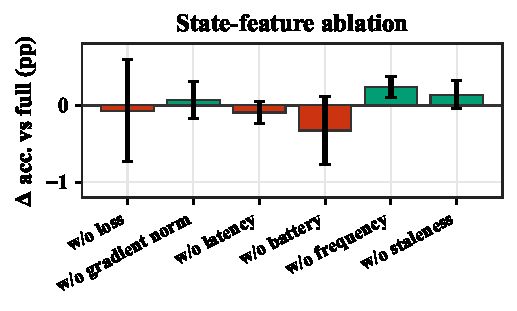
\includegraphics[width=0.6\textwidth]{images/fig_feature_ablation_trimmed_boxed.pdf}
\end{center}
\noindent\emph{Change in final accuracy on Fashion-MNIST when each feature is removed in turn. Removing the battery feature causes the largest drop, confirming that both learning and system signals are used.}
}

\noindent

\textbf{Comment 9:} \textit{Fig. 2 has small font sizes and unclear
axis scaling.} 

\noindent

\textbf{Reply 9:}{We thank the reviewer for comment. In
the revised manuscript, the font size and the font has been kept same
as the text size and font. Axis are also defined clearly with their
symbols and units. Specifically, the figure text now matches the manuscript body text in both font family and size, neither larger nor smaller.
 The convergence figure (Fig.~2) is now at full column width. The
subfigures report CIFAR-100 test accuracy, the selector meta-update
magnitude $\lVert\phi_{t+1}-\phi_t\rVert_2$ (policy stabilization), cumulative
modelled energy, and test loss over rounds. }

\noindent

\textbf{Comment 10:} \textit{The definition of ``Time (Units)''
is unclear.} 

\noindent

\textbf{Reply 10:}{We thank and agree with the reviewer
regarding the unit of time. In the updated paper, this time unit
is removed. The results table (Table~II) now reports only well-defined
quantities. These are accuracy, weighted precision, recall, F1, TFLOPs,
modelled energy (Wh), Jain fairness,
and coverage. The round latency is described through the straggler-bound
round time in the System Model.}

\noindent

\textbf{Comment 11:} \textit{Include recent baselines such as
CriticalFL and FedGCS.} 

\noindent

\textbf{Reply 11:}{We thank the reviewer for suggesting
the two baselines. In the revised manuscript, we have now added the
comparison with both the suggested methods. FedGCS uses generative
client-combination search, whereas CriticalFL uses critical-period
cohort scaling. Both are also now in the comparison Table - I, the
related-work discussion, and the main evidence figures (Figures 2
and 3). The comparison in simulation now consists of eight methods
in total, that is, FedAvg, FedCS, Oort, TiFL, FedCor, FedGCS, CriticalFL,
and the proposed MAML-Select. Their client selection strategies span
over a wide variety, including random, system-aware, utility-aware,
correlation-based, generative, and critical-period selection. Therefore,
the evaluation now places MAML-Select against current state-of-the-art
selectors.}

\noindent

\textbf{Comment 12:} \textit{Proofread the manuscript for grammar,
punctuation, and sentence structure.} 

\noindent
\textbf{Reply 12:} {Thanks for the comment. In the revised
version, we have significantly updated the manuscript, and revised
multiple times to avoid grammatical, punctuation and sentence errors.
The Abstract, Impact Statement, Introduction, Related Work, Methodology,
Evaluation, and Conclusion were all edited for clarity and consistent
terms.}\\

\hspace{0.75cm}{\bf {\Large {~~~~~~~~~~~~Response to Comments of Reviewer 3}}}

\noindent
\textbf{Comment 1:} \textit{The motivation is not clear.} 

\noindent
\textbf{Reply 1}{We thank the Reviewer for pointing out
the motivation. In the revised version, the manuscript is significantly
enhanced including the motivation. The main motivating factor in this
work is the non-stationary behavior of client selection utility in
federated learning. A client that is useful in one round may be less
useful later. The reason is that many things change during training,
including the global model, the local loss, the device latency, battery
state, the participation history. A fixed scoring rule cannot track
this drift. Re-training a heavy controller from scratch each round
is also impractical at the edge. The proposed MAML-Select solves this
by meta-learning a ranking policy. Its initialization can be adapted
with a single gradient step. This step uses the most recent round's
feedback, just before the next decision. Thus, the proposed method
is fast enough to run every round, and is also responsive to the changing
utility. This motivation is now updated in the Abstract and the Introduction.}

\noindent
\textbf{Comment 2:} \textit{Highlight the novelty and main contribution.} 

\noindent
\textbf{Reply 2:} {We thank the reviewer for the comment.
In the significantly revised version of the manuscript, we have stated
the contribution more precisely and clearly in the introduction section.
To the best of authors' knowledge, the proposed method is the first
one to treat per-round federated client selection as a meta-learning
task, and to solve it with first-order MAML. Among the novelty and
contribution, the following are main contributing factors. First,
the meta-learned object is the server-side ranking policy, not the
client model. Thus, this MAML model is not for personalization of
clients model. Second, each round is treated as a task and has an
explicit support set, which is the previous round's selected-client
feedback. Each round also has a query set, which is the current candidate
pool. Thus, the policy is re-fitted by a gradient step right before
every selection. Third, the cost that supervises the policy joins
learning progress and system latency using the weight parameter, $\lambda$,
which enables a tunable computational and energy efficiency and accuracy
operating point. The following has been updated in the revised version
as follows:

``\emph{The major contributions can be summarized as follows.}

\emph{1) We formulate the FL client selection problem as a meta-learning
task and introduce the MAML-Select algorithm with rapid gradient-based
adaptation for online client selection.}

\emph{2) Experiments on Fashion-MNIST, CIFAR-10, and CIFAR-100 under
non-IID settings (\textgreek{α} = 0.5, three seeds) show that MAML-Select
delivers accuracy competitive with FedAvg and FedGCS at lower computational
cost, and higher accuracy than FedCS, Oort, TiFL, and FedCor; sensitivity
and ablation studies over \textgreek{λ}, the inner-loop steps, the
selector width, and}

\emph{the state features support the design choices.}

\emph{3) We demonstrate that MAML-Select lowers cumulative training
TFLOPs by up to 21.5\% and modelled energy by up to 24.7\%
relative to FedAvg, with paired-test support for the resource reductions.}''

Moreover, in the the section ``Related work'', the subsection ``Difference
from prior work'' paragraph is added, and Table~I now make this
three-part contribution explicit. }

\noindent
\textbf{Comment 3:} \textit{Add appropriate constraints to the
problem formulation.} 

\noindent
\textbf{Reply 3:} {We thank the reviewer for pointing out
the constraints in the problem formulation. In the equation (3) in
the section III in the revised version, we have added the missing/implicit
constraints, so the selection problem is fully specified as 
\begin{equation}
\begin{aligned}\min_{\pi_{\phi}}\quad & \sum^{T}_{t=1}\left[F(\theta_{t+1})+\lambda T^{round}_{t}\right]\\
\text{subject to} & \sum^{N}_{i=1}a_{i,t}=K,\forall a_{i,t}\in\{0,1\},\\
 & a_{i,t}\leq\mathbf{1}\{i\in\mathcal{A}_{t}\}.
\end{aligned}
\end{equation}
The System Model now introduces the per-round available-client set
$\mathcal{A}_{t}$. It adds binary decision variables $a_{i,t}\in\{0,1\}$.
It adds the cohort-size constraint $\sum_{i}a_{i,t}=K$. It adds the
availability constraint $a_{i,t}\le\mathbf{1}\{i\in\mathcal{A}_{t}\}$,
with $\mathcal{S}_{t}=\{i:a_{i,t}=1\}$. It can be seen that the client
selection is a combinatorial choice, and made over a small feasible
cohort.}

\noindent
\textbf{Comment 4:} \textit{Why is only one method considered
as a baseline? Consider at least two more baselines.} 

\noindent
\textbf{Reply 4:} {We thank the reviewer for the comment.
In the updated manuscript, the revised evaluation now compares the
proposed MAML-Select against seven other baselines algorithms. FedAvg
has random client selection. FedCS is system-aware and deadline-constrained
client selection. The client choosing in the Oort uses utility-based
importance sampling. TiFL adopts a tier-based approach to trim the
clients. FedCor employs correlation-based client filtering, using
Gaussian Processes. FedGCS utilizes generative methods to include
and exclude clients. CriticalFL uses critical-period cohort scaling.
All of these methods appear in Table~II, the related-work comparison
(Table~I), and the main evidence figures (Figure 2 and 3). Therefore,
the comparison is now broad, not single-baseline.}

\noindent
\textbf{Comment 5:} \textit{Provide more simulation results to
ensure effectiveness.}

\noindent
\textbf{Reply 5:} {We thank the reviewer for the comment.
In the revised simulations, we have now expanded the empirical evidence
to a great deal. The revised paper covers three datasets and 7 other
baselines. Fashion-MNIST and CIFAR-10 run for $200$ rounds. CIFAR-100
runs for $150$ rounds. The new simulations covers eight methods and
three seeds, with mean\,$\pm$\,std and paired-test significance.
Fairness and coverage metrics are also added. A two-dataset $\lambda$
sweep is also added. Energy in terms of computational overhead is added. A supporting complexity result is added
to provide selector-overhead scaling study. The reported metrics include
accuracy, precision, recall, F1, compute, energy, fairness,
coverage, sensitivity, ablation, and server-side overhead. More tables
and figures are in the Supplementary Material (Sections~S2 to~S5).}

\noindent
\textbf{Comment 6:} \textit{Remove references from the conclusion
and write the conclusion as a concise single paragraph.} 

\noindent
\textbf{Reply 6:}{We thank and agree with the reviewer's
comment. The Conclusion section is now a single concise paragraph
with no citations. It summarizes the method and findings. It ends
with a short statement of future directions. These are a broader evaluation
across heterogeneity levels, client-pool sizes, and naturally federated
benchmarks, an asynchronous extension, and a differentially private
treatment of the client-state vector.}

\hspace{0.75cm}{\bf {\Large {~~~~~~~~~~~~Response to Comments of Reviewer 4}}}

\noindent
\textbf{Comment 1:} \textit{Correct the Impact Statement wording
for heterogeneous environments and industrial Internet of Things.}\\
\noindent
\textbf{Reply 1:} We thank the reviewer for the suggestion. The Impact Statement has been revised to incorporate the recommended terminology for heterogeneous environments and the industrial Internet of Things.

\noindent
\textbf{Comment 2:} \textit{Improve long sentences, grammar, and
proofreading throughout the manuscript.} \\
\noindent
\textbf{Reply 2:} {We thank the reviewer for the comment. The manuscript is significantly revised for towards readability of long sentences and grammar. The revised paper has been proofread multiple times by all the authors. The Abstract, Impact Statement, Introduction, Related Work, Methodology, Evaluation, and Conclusion were all edited, in response to the comments by the Reviewer~1, Comment~1, and Reviewer~2,Comment~12. We hope this improved version will have much better readability.
}

\noindent
\textbf{Comment 3:} \textit{Update the literature review with
recent and related papers.} \\
\noindent
\textbf{Reply 3:} We thank the reviewer for the insightful comment. We have updated the Related Work section with recent and relevant studies. The newly added references and corresponding discussion have been marked in blue in the revised manuscript.

\noindent
\textbf{Comment 4:} \textit{Include a comparison table with previous state-of-the-art works.}\\
\noindent
\textbf{Reply 4:} {We thank the reviewer for the suggestion.
In the revised version, we have added the Table~I, which compares
representative client-selection and meta-learning approaches against
MAML-Select. It uses four columns: primary objective, adaptation mechanism,
selection complexity or dominant server-side operation, and optimization
strategy, which makes the proposed method's position relative to prior
work clear at a glance.}

\noindent
\textbf{Comment 5:} \textit{Make the Conclusion and Future Work
section accurate and concise. Avoid too many citations.}\\
\noindent
\textbf{Reply 5:} {We thank the reviewer for the comment.
The Conclusion section is now revised to a single concise paragraph without citations. The section ends with a short paragraph of future directions.}

\noindent
\textbf{Comment 6:} \textit{Fig. 2 requires clarification, justification, and a clearer comparison with other schemes.}\\
\noindent
\textbf{Reply 6:} {We thank the reviewer for the comment
mentioning the justification. In the revised manuscript, the Figure
2 (the original single-curve figure in the old manuscript) has been
replaced by clearer and multi-metric evidence. The figure 2 now reports
CIFAR-100 accuracy, the selector meta-update magnitude (policy stabilization),
cumulative modeled energy, and testing loss over rounds; the accuracy,
energy, and loss panels cover all eight methods. The efficiency and accuracy
trade-off figure is depicted in Fig.~3(a), in which MAML-Select
is compared directly against every baseline. Figure 3 uses final accuracy
and training computational cost relative to the FedAvg method. The revised Fig.~2 is shown below.

\begin{center}

\includegraphics[width=0.97\textwidth]{images/fig_convergence_boxed.pdf}
\end{center}
\noindent{Revised Fig.~2: CIFAR-100 test accuracy, selector meta-update magnitude (policy stabilization), cumulative modelled energy, and test loss over communication rounds; the accuracy, energy, and loss panels cover all eight methods.}
}
\end{document}


